\section{Terapie}
Sono numerose le malattie che possono danneggiare i reni ed alcune di queste portano inesorabilmente alla perdita della loro funzionalità. Quando questo avviene le uniche possibilità terapeutiche per il paziente sono il trapianto di rene e la dialisi.

\subsection{Trapianto}
L'intervento chirurgico di trapianto prevede l'anastomosi dei vasi del rene con i vasi iliaci del ricevente e l'attacco del'uretere, proveniente dallo stesso donatore, alla vescica. Come è necessario nel caso di tutti i trapianti di organo o tessuto, anche nel caso del trapianto di rene, per preservare l'integrità dell'organo trapiantato, devono essere somministrati farmaci immunosoppressori per evitarne il rigetto. I pazienti trapiantati sono in grado di reinserirsi pienamente nel contesto sociale di cui facevano parte prima della malattia.

Il trapianto di rene può essere eseguito prelevando l'organo da cadavere o da un donatore vivente. Il vantaggio del trapianto di rene da donatore vivente è legato alla sua programmabilità e ad una probabilità di successo lievemente superiore al trapianto da donatore cadavere.  L'individuo che volontariamente si offre ad una donazione di rene esegue una serie di accertamenti che mirano ad escludere la possibilità che egli stesso abbia una nefropatia latente o una patologia che favorisca uno sviluppo di nefropatia, in modo da proteggerlo, nonostante il prelievo del rene, da un possibile danno futuro. L'atto chirurgico del prelievo del rene può essere eseguito in chirurgia laparoscopica e quindi con minima invasività.



\subsection{Dialisi}
In generale per dialisi si intende un processo di purificazione di un fluido per mezzo di un'altro fluido, detto dializzante, separato dal primo attraverso una membrana semipermeabile artificiale o biologica. A seconda della tecnica di dialisi, gli scambi di massa attraverso la membrana avvengono per diffusione e/o convezione.

\subsubsection{Dialisi peritoneale}
\begin{wrapfigure}{O}{0.32\textwidth}
	\centering
	\vspace{-20pt}
		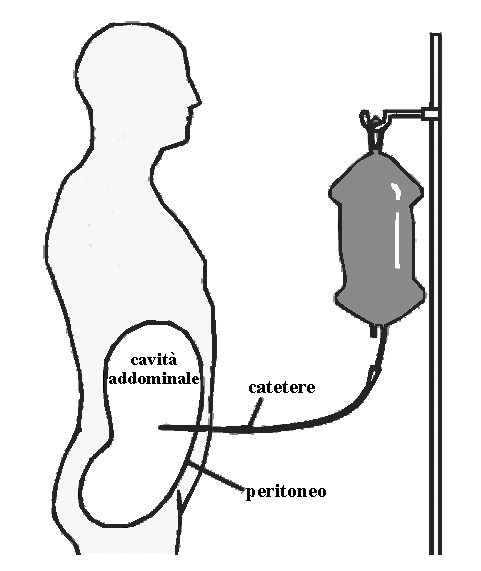
\includegraphics[width=0.32\textwidth]{immagini/peritoneale.eps}
		\vspace{-20pt}
\end{wrapfigure}
La dialisi peritoneale fa uso del peritoneo come membrana semipermeabile. Quando si riempie l'addome col liquido dializzante, si instaura uno scambio diffusivo di soluti fra i vasi del peritoneo e la cavità addominale. È anche possibile, oltre ai cataboliti, estrarre fluidi corporei in eccesso (ultrafiltrazione) giocando sull'osmolarità del liquido dializzante. Il dializzante è mantenuto nella cavità addominale per il tempo necessario agli scambi. Il ciclo è ripetuto fino a dieci volte al giorno, talvolta con l'ausilio notturno di un dispositivo automatico per il riempimento e svuotamento dell'addome. Questa tecnica \textit{auto-terapica} richiede molta diligenza da parte del paziente, ma facendo uso di dispositivi semplici e poco ingombranti, dà una maggiore libertà di programmazione delle sedute dialitiche anche lontano da centri specializzati.
 

\subsubsection{Emodialisi}

\begin{wrapfigure}{O}{0.32\textwidth}
	\centering
	\vspace{-20pt}
		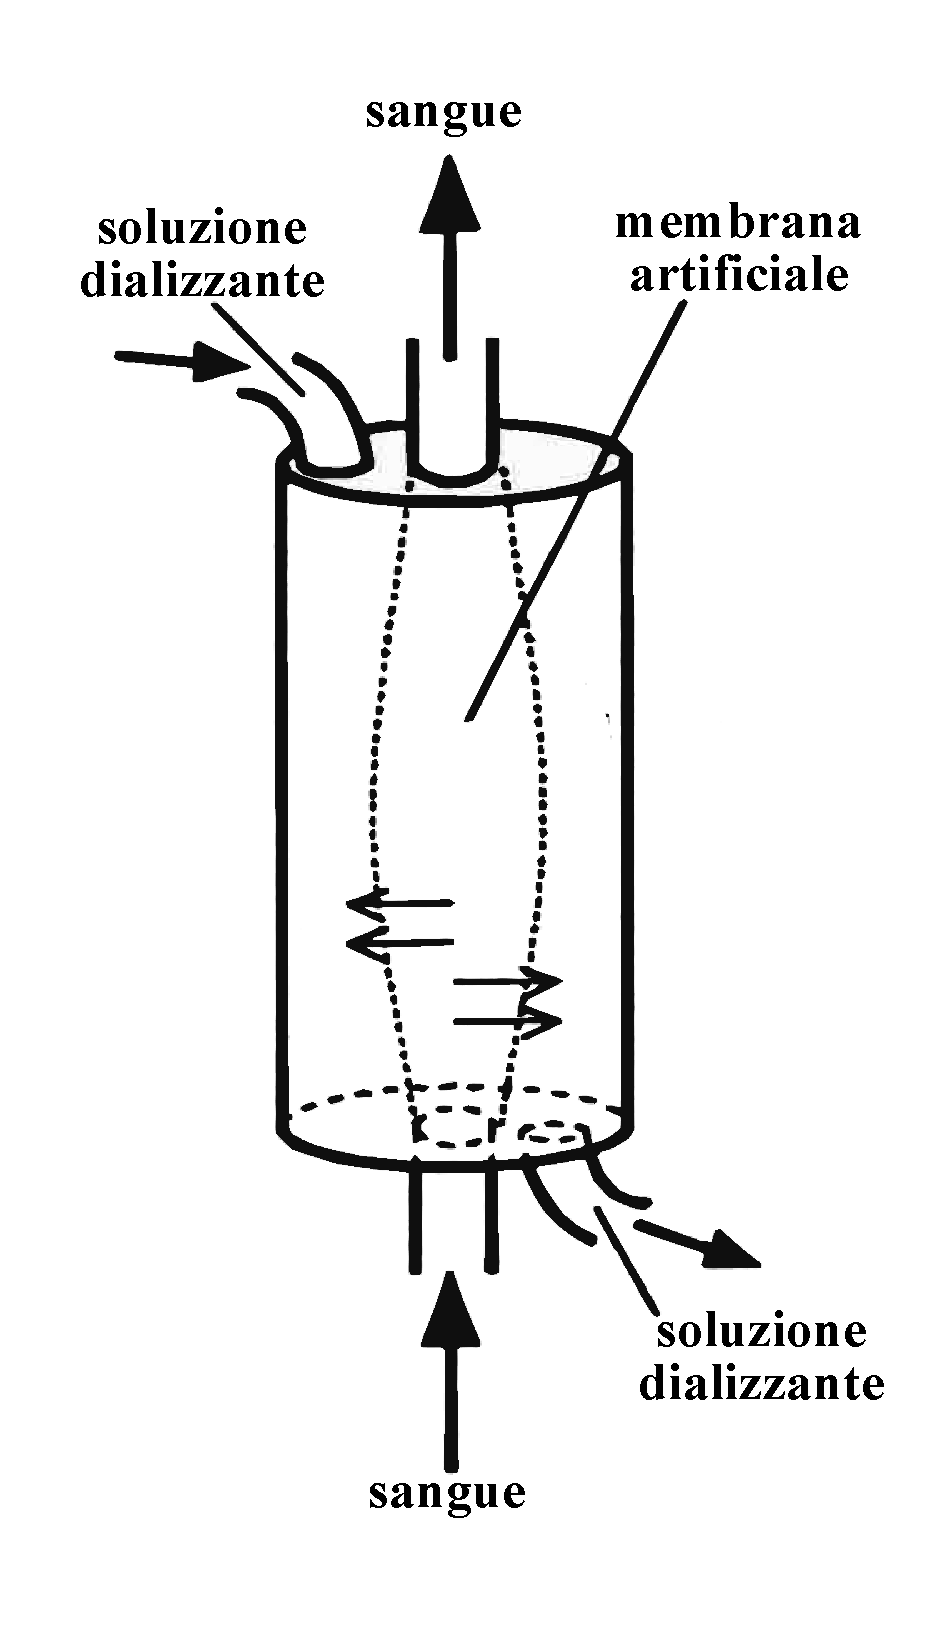
\includegraphics[width=0.32\textwidth]{immagini/emod.eps}
		\vspace{-20pt}
\end{wrapfigure}

L'emodialisi (HD) è una terapia che permette di purificare il sangue del paziente tramite un dializzatore, ovvero rene artificiale. Diversamente dal rene biologico che è in grado anche di riassorbire attivamente sostanze di cui si vuole evitare la perdita, il rene artificiale esercita sulla composizione del plasma un ruolo puramente passivo. La funzione di eliminazione delle sostanze di scarto (urea, creatinina ed altre) viene eseguita semplicemente ponendo a contatto, tramite una membrana artificiale, il sangue da filtrare con una soluzione dializzante di composizione uguale a quella che normalmente dobrebbe avere il plasma.

Il dializzatore è costituito da una membrana semipermeabile artificiale che trattiene i globuli rossi e le proteine del plasma e permette la diffusione delle molecole di scarto, a basso peso molecolare, dal plasma al liquido dializzante, per cui la concentrazione dei soluti di scarto nel plasma, elevata all'inizio della dialisi, diminuisce nel corso della dialisi. Le molecole necessarie all' organismo non vengono eliminate, poiché sono presenti, in concentrazione fisiologica, nella soluzione dializzante. Inoltre un soggetto uremico non ha la possibilità di eliminare, per vie naturali, anche i liquidi, i quali tendono ad accumularsi nell 'organismo nella quantità di circa un litro al giorno, col rischio di provocare un edema polmonare dopo alcuni giorni. Perciò nell'emodialisi è necessario mantenere una modesta differenza di pressione idraulica tra i due compartimenti, in modo che parte del solvente (acqua) dal sangue attraversi la membrana e venga eliminata. Al processo di diffusione allora si aggiunge, seppur con effetto trascurabile,  anche quello di convezione. La quantità di acqua così eliminata, circa mezzo litro l'ora, deve essere controllata, nel corso della dialisi, insieme alle condizioni generali del paziente, poiché una brusca e notevole disidratazione può portare al collasso con successive gravi conseguenze.

\subsubsection{Emofiltrazione}
L'emofiltrazione (HF) è una tecnica dialitica che permette la rimozione di soluti quasi esclusivamente per convezione. Grazie infatti all'alta porosità delle membrane qui usate, applicando un'adeguata pressione di trans-membrana, è possibile rimuovere un elevato volume di acqua, dell'ordine della decina di litri a seduta, che trasporta con sè le sostanze in essa disciolte; poiché una perdita così elevata di fluidi non è sostenibile dall'organismo umano, è necessario rimpiazzare la maggior parte del volume filtrato con un adeguato flusso di liquido di sostituzione, ovvero di diluizione, a monte o a valle rispetto al dializzatore, cioè in pre- o post-diluizione. Dovrà quindi essere aggiunto ad un normale circuito di dialisi un ulteriore circuito per la somministrazione della soluzione nel lato sangue. La porosità della membrana è un parametro importante nel trasporto per convezione, poiché in questo modo è possibile rimuovere prodotti di scarto di dimensioni più elevate, cosa che con l'emodialisi non può accadere.

\subsubsection{Emodiafiltrazione}
Il termine \textit{emodiafiltrazione} (HDF) fu utilizzato per la prima volta da Leber et al. \cite{leber} in Germania e fu proposto come un nuovo metodo per la purificazione del sangue ottenuta tramite la combinazione equilibrata di diffusione e convezione.
L'HDF può difatti essere definita come una tecnica di dialisi che utilizza membrane altamente permeabili, nelle quali la diffusione e la convezione sono equamente determinanti per la rimozione di soluti/tossine di vario peso molecolare.
Uno dei grandi risultati dell'HDF è infatti quello di poter rimuovere non solo soluti a basso peso molecolare, come accade per l'emodialisi, ma anche molecole ritenute dannose, come le $\beta_2$-microglobuline ($11,8$ $kDa$), che fanno parte della categoria delle sostanze a medio/alto peso molecolare.

Inizialmente nella dialisi erano i soli processi diffusivi a regolare la purificazione del sangue e ciò a causa della bassa permeabilità idraulica delle membrane e una porosità insufficiente a permettere alti flussi,. Grazie allo sviluppo di polimeri sintetici con una struttura ibrida idrofilica e idrofobica,e uno spessore di membrana ridotto si è potuto sfruttare anche il processo convettivo di purificazione ematica e dare quindi il via alla tecnica dell'emodiafiltrazione.

Nell'HDF  il trasporto di soluti può avvenire e per diffusione e per convezione. Il trasporto diffusivo è governato dalla legge di Fick, espressa matematicamente da $$J_d = -D_s \frac{dC_s}{dx}$$
dove $J_d$ è il flusso netto diffusivo, $D_s$ il coefficiente di diffusione del soluto in esame e $C_s$ la sua concentrazione.
Il trasporto convettivo è invece caratterizzato dalla filtrazione di fluido attraverso la membrana come conseguenza di un gradiente locale di pressione, in formule:
$$J_t = L_p (\Delta P - \Delta\Pi)\overline{C}_s$$
dove $L_p$ è la permeabilità idraulica della membrana, $\Delta P$ il gradiente idraulico e $\Delta \Pi$ il gradiente osmotico a cavallo della membrana e  $\overline{C}_s$ la concentrazione media di membrana del soluto trasportato.
Esiste infine un altro fenomeno utile alla rimozione di soluti in HDF e si tratta dell'\textit{adsorbimento}. Questa modalità è utilizzata anche in un dispositivo, del tutto analogo a un dializzatore, per filtrare il liquido di dialisi una o più volte e renderlo ultrapuro prima del suo utilizzo.

L'efficienza dell'HDF è influenzata, come per l'emodialisi, dalla tipologia di flusso del sangue e del liquido di dialisi e dalla concentrazione dei globuli rossi. L'efficienza dell'HDF dipende anche dalla modalità di infusione del fluido di sostituzione: pre-diluizione e post-diluizione. A parità di altre condizioni, in post-diluizione la \textit{clearance} delle molecole a basso/medio peso molecolare è maggiore rispetto all'emodialisi. Il sangue però rischia di coagulare all'interno del dializzatore, a seguito dell'aumento di ematocrito che si verifica lungo i capillari. In pre-diluizione invece il sangue ha prorpietà reologiche meno favorevoli alla coagulazione, ma a causa della diluizione preventiva la cleareance dei soluti ne risulta diminuita.


\subsubsection{Tipologie di HDF}
L'emodiafiltrazione è una combinazione di emodialisi e emofiltrazione che rende possibile la rimozione simultanea di soluti a basso e alto peso molecolare. Il contributo relativo della convezione rispetto alla diffusione, aumenta all'aumentare del peso molecolare del soluto da rimuovere. Questi concetti sono stati implementati nella pratica clinica attraverso a diverse tipologie di HDF, descritte da C.Ronco~\cite{evolutionHDF}, che illustreremo nei prossimi paragrafi.


\paragraph{HDF classica.}
Questa tipologia è caratterizzata da portate di reinfusione di circa $3$-$15$~$L/seduta$ tipicamente in post-diluizione. Il liquido di diluizione è contenuto in apposite sacche sterili. Per ottenere un livelli accettabili di ultrafiltrazione e regimi pressori trans-membranici, sono necessarie portate di sangue superiori ai $300$~$mL/min$. Questa tecnica è stata utilizzata per molti anni, prima che fossero disponibili modalità di produzione \textit{on-line} del fluido di diluizione, economicamente più vantaggiose.

\paragraph{On-line HDF.}
A causa dell'elevato costo delle soluzioni di reinfusione e grazie al miglioramento delle tecnologie per la preparazione del liquido di dialisi è stato possibile sviluppare una nuova tecnica chiamata \textit{on-line} HDF. In questa modalità, una certa quantità di dialisato ultrapuro è preparato al momento dalla macchina dializzatrice. La qualità del fluido prodotto è eccellente, ed è garantita dalla ridondanza dei sistemi di filtraggio. La concentrazione dei soluti nel dialisato è controllata dal software della macchina attraverso celle conduttimetriche. Questo procedura rende disponibile immediatamente e a basso costo una grande quantità di liquido di sostituzione e l'HDF può essere portata a termine con un elevato ricambio di fluido (intorno ai $40$~$L/sessione$) utilizzando la pre- o la post-diluizione o, ancora in fase sperimentale \cite{pedrini}, un mix delle due modalità.

\paragraph{Internal-Filtration HDF.}
Quando un dializzatore ad alta permeabilità è usato in condizioni di minima ultrafiltrazione, intuitivamente si pensa che il processo di scambio savvenga per pura diffusione come nel caso dell'emodialisi. Ciò è incorretto. In effetti gli scambi convettivi, mascherati dalla cinetica interna della \textit{retro-filtrazione}, non sono affatto trascurabili. Il fenomeno è del tutto paragonabile a ciò che avviene nel letto capillare umano secondo l'ipotesi di Starling (\figurename\ref{starling}): man mano che si avanza nel lato sangue lungo i capillari, la pressione idraulica diminuisce fino al punto in cui è possibile che la pressione di trans-membrana si inverta, richiamando liquido dializzante nel lume ematico. Questo fenomeno può essere amplificato ragionando sulle implicazioni della legge di \textit{Poiseuille} (equazione~(\ref{Qt})) applicando, per esempio, una restrizione verso la metà del fascio di capillari, oppure riducendo il diametro interno delle fibre. In questo modo la retro-filtrazione può raggiungere valori di $40$-$50$ $mL/min$ con un dializzatore da $1.8$~$m^2$ in regime di ultrafiltrazione netta nulla.
Anche se questo fenomeno avviene in qualsiasi dializzatore ad alta permeabilità, quando specifici accorgimenti e particolari design del dializzatore sono usati per favorire la retro-filtrazione la tecnica dialitica prende il nome di internal-HDF.

\paragraph{Paired Filtration.}
Questa tipologia di HDF è stata concepita per la prima volta in Italia. È caratterizzata da due dializzatori posti in serie: il primo molto poroso in cui è dominante la convezione, il secondo un classico emodializzatore nel quale è la diffusione il fenomeno preponderante. Il fluido di diluizione è immesso nel circuito tra un filtro e l'altro. Lo scopo di questo design è quello di minimizzare le interazioni sfavorevoli tra convezione e diffusione, di prevenire la retro-filtrazione e di ottenere misure più accurate sull'ultrafiltrato essendo questo provvisto di una linea separata dalla linea di uscita del dialisato.

\paragraph{Mid-diluition HDF.}
Per questo tipo di HDF è necessario un filtro particolare costituito da due compartimenti longitudinali posti idraulicamente in serie. Il sangue entra nel primo compartimento in contro-corrente al dialisato; qui avviene l'ultrafiltrazione. Quando il sangue emoconcentrato giunge alla fine del primo compartimento è diluito col fluido di sostituzione e immesso nel secondo compartimento iso-corrente al dialisato. Il sangue in uscita lascia il dializzatore da una porta vicina a quella di ingresso.

\paragraph{Double High-Flux HDF.}
si utilizzano due dializzatori ad alta porosità posti in serie. La filtrazione avviene nell'unità prossimale e la retro-filtrazione in quella distale. La retro-filtrazione, ovvero la portata del fluido di diluizione, può essere modulata da una resistenza idraulica posta sulla linea del dialisato congiungente i dializzatori. Quando si riescono a raggiungere alti flussi di fistola ($>500$~$mL/min$) l'alta efficienza di questa metodologia permette trattamenti della durata inferiore alle due ore \cite{miller}.

\paragraph{Push-Pull HDF.}
Con questa tecnica è possibile variare il rapporto fra filtrazione e retro-filtrazione. La rotazione della pompa pre-filtro (mentre quella post-filtro è ferma) produce filtrazione; la rotazione della pompa post-filtro (mentre è ferma quella pre-filtro) genera una pressione negativa nel compartimento ematico e quindi retro-filtrazione. Le pompe di modulazione possono in alternativa essere poste sulla linea del dialisato.

\begin{figure}[htb]
	\centering
	\subfigure[]%
	{
\includegraphics[width=0.45\textwidth]{immagini/classicHDF.eps}}\qquad
	\subfigure[]%
	{
\includegraphics[width=0.45\textwidth]{immagini/onlineHDF.eps}}\\
	\subfigure[]%
	{
\includegraphics[width=0.45\textwidth]{immagini/paired.eps}}\qquad
	\subfigure[]%
	{
\includegraphics[width=0.45\textwidth]{immagini/midHDF.eps}}\\
		\subfigure[]%
	{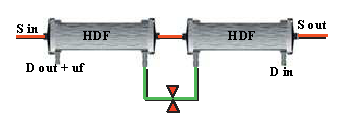
\includegraphics[width=0.45\textwidth]{immagini/doubleHDF.eps}}\qquad
	\subfigure[]%
	{
\includegraphics[width=0.45\textwidth]{immagini/pushpull.eps}}
	\caption{Differenti modalità di emodiafiltrazione. (a) HDF classco, (b) on-line HDF, (c) paired HDF, (d) mid-diluition HDF, (e) double high-flux HDF, (f) push-pull HDF.}\label{evolution}		
\end{figure}